\section{Инсталација   \textit{Lustre} фајл система}
\subsection{Инсталација оперативног система}

Да би се инсталирао \textit{Lustre} фајл систем, потребно је имати најмање 3, а пожељно је имати 4 чвора. 

За ову инсталацију користи се \textit{Xubuntu} 14.04 оперативни систем на којем је инсталиран \textit{VirtualBox} 4.3.10, помоћу којег се креирају 4 виртуалне машине(слика 2.5). Свакој машини је потребно доделити 768MB RAM меморије и 1 процесор.
\begin{figure}[h!]
  \centering
      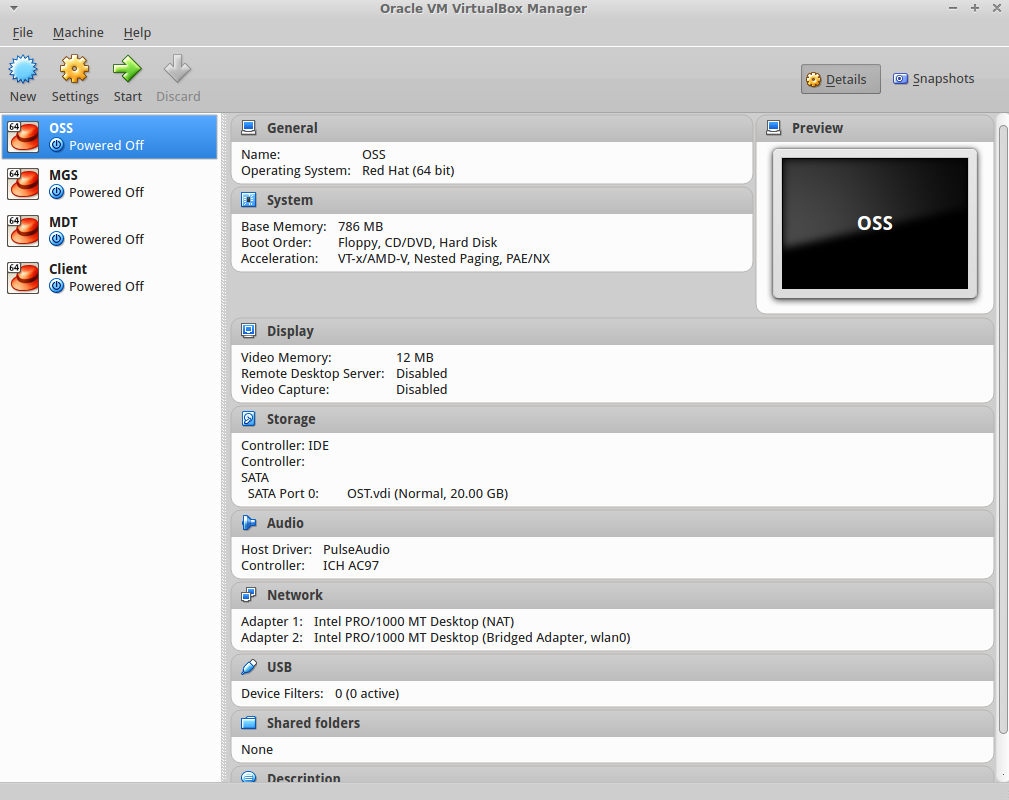
\includegraphics[width=1\textwidth]{slike/virtualbox.png}
  \caption{Bиртуалне машине}
\end{figure}
Да би машина имала приступ интернету, потребно је у подешавањима, у секцији \textit{Network} поставити први адаптер на \gls{NAT}, a други на \textit{Bridged Adapter}. 	\textit{Bridged Adapter} је потребан да би машине комуницирале у локалној мрежи.
~\\[3cm]
На свим чворовима биће инсталиран \textit{Scientific Linux 6.5} и сваком чвору бити додељена по једна статичка IP адреса(Табела 2.1).
\begin{center}
\captionof{table}{Тестна конфигурација   \textit{Lustre} чворова}
    \begin{tabular}{ | l | l | l | p{5cm} |}
    \hline
    \textbf{Оперативни систем} & \textbf{Назив} & \textbf{IP } & \textbf{Функција} \\ \hline
Scientific Linux 6.5 & mgs &  192.168.1.200 & Managment Server \\ \hline
Scientific Linux 6.5 & mdt &  192.168.1.201 & Metadata Server \\ \hline
Scientific Linux 6.5 & oss &  192.168.1.202 & OS Server \\ \hline
Scientific Linux 6.5 & client &  192.168.1.203 & Client \\ \hline
    \end{tabular}

\end{center}

На MGS-у, MDT-у и OSS-у чврсти диск је подељен на:
\begin{itemize}
\item \textit{Boot} партиција – 10 GB (\textit{root}, \textit{home} директоријум)

\item \textit{Swap} партиција – 2 GB

\item Logical volume partition – 8 GB ( \gls{LVM} партиција за   \textit{Lustre} фајл систем)
\end{itemize}


Након инсталације оиперативног система, потребно је урадити следеће кораке:

\begin{enumerate}
\item  Обезбедити SSH приступ између свих машина. 
SSH daemon се стартује командом
\begin{verbatim}
/etc/init.d/sshd start
\end{verbatim}
док следећом командом подешавамо да се  SSH сервис покреће приликом подизања оперативног система
\begin{verbatim}
chkconfig sshd on
\end{verbatim}

\item Инсталација потребних програма

Да бисмо касније компајлирали кернел, потребни су пакети попут \textit{gcc, make} ... Њих инсталирамо командом:

\begin{verbatim}
yum -y groupinstall "Development Tools"
\end{verbatim}

\item Додавање  IP адреса у \textit{/etc/hosts} фајл. На свим чворовима додати следеће линије у \textit{/etc/hosts} фајл:
\begin{verbatim}
192.168.1.200   mgs
192.168.1.201   mdt
192.168.1.202   ost
192.168.1.203   client
\end{verbatim}

\item  Искључити  \textit{Linux Firewall}
\begin{verbatim}
chkconfig iptables off
\end{verbatim}

\item Потребно је скинути    \textit{Lustre} пакете(Листинг 2.3).
\begin{lstlisting}[style=nonumbers,frame=single, caption= \textit{Lustre} пакетi]
cd  /home/mgs/Downloads/

wget http://downloads.whamcloud.com/public/lustre/latest-maintenance-release/el6/server/RPMS/x86_64/
kernel-2.6.32-358.23.2.el6_lustre.x86_64.rpm

wget http://downloads.whamcloud.com/public/lustre/latest-maintenance-release/el6/server/RPMS/x86_64/
kernel-firmware-2.6.32-358.23.2.el6_lustre.x86_64.rpm

wget http://downloads.whamcloud.com/public/lustre/latest-maintenance-release/el6/server/RPMS/x86_64/
lustre-2.4.2-2.6.32_358.23.2.el6_lustre.x86_64.x86_64.rpm

wget http://downloads.whamcloud.com/public/lustre/latest-maintenance-release/el6/server/RPMS/x86_64/
lustre-ldiskfs-4.1.0-2.6.32_358.23.2.el6_lustre.x86_64.x86_64.rpm

wget http://downloads.whamcloud.com/public/lustre/latest-maintenance-release/el6/server/RPMS/x86_64/
lustre-modules-2.4.2-2.6.32_358.23.2.el6_lustre.x86_64.x86_64.rpm

wget http://downloads.whamcloud.com/public/lustre/latest-maintenance-release/el6/server/RPMS/x86_64/
lustre-osd-ldiskfs-2.4.2-2.6.32_358.23.2.el6_lustre.x86_64.x86_64.rpm

wget http://downloads.whamcloud.com/public/e2fsprogs/latest/el6/RPMS/i686/e2fsprogs-1.42.7.wc2-7.el6.i686.rpm

wget http://downloads.whamcloud.com/public/e2fsprogs/latest/el6/RPMS/i686/e2fsprogs-libs-1.42.7.wc2-7.el6.i686.rpm

wget http://downloads.whamcloud.com/public/e2fsprogs/latest/el6/RPMS/i686/libss-1.42.7.wc2-7.el6.i686.rpm

wget http://downloads.whamcloud.com/public/e2fsprogs/latest/el6/RPMS/i686/libcom_err-1.42.7.wc2-7.el6.i686.rpm
\end{lstlisting}

\item Ископирати пакете на OSS i MDT помоћу команде \texttt{scp}:
\begin{verbatim}
scp -r /home/mgs/Downloads/ ost:/home/ost/
scp -r /home/mgs/Downloads/ mdt:/home/mdt/
\end{verbatim}

\item Креирати фајл \textit{/etc/modprobe.d/lustre.conf} и подесити мрежни протокол и мрежно окружење додавањем следеће линије:
\begin{verbatim}
	options lnet networks=tcp0(eth1)
\end{verbatim}

\item Такоће, ископирати \textit{lustre.conf} на OSS i MDT:
\begin{verbatim}
scp  /etc/modprobe.d/lustre.conf mdt:/etc/modprobe.d/lustre.conf
scp  /etc/modprobe.d/lustre.conf ost:/etc/modprobe.d/lustre.conf
\end{verbatim}

% MИЛОШ: Зашто овде кажеш да се кернел компајлира??? Исправио сам у "инсталирати".
\item Инсталирати \textit{Lustre} кернел:
\begin{lstlisting}[style=nonumbers,frame=single, caption=Инсталација \textit{Lustre} кернела]
rpm -ivh kernel-2.6.32-358.23.2.el6_lustre.x86_64.rpm  kernel-firmware-2.6.32-358.23.2.el6_lustre.x86_64.rpm 
\end{lstlisting}
\item Инсталирати \textit{e2fsprogs} 
\textit{e2fsprogs} је скуп програма за одржавање \textit{Linux} фајл система. \textit{e2fsprogs} садржи неколико програма од којих су најпознатији:

\begin{itemize}
\item \textbf{\textit{e2fsck}} - Проверава и поправља несугласице.
\item \textbf{\textit{mke2fs}} - Креирa ext2, ext3 и ext4 фајл системe.
\item \textbf{\textit{resize2fs}} - Промена величине фајл система.
\item \textbf{\textit{tune2fs}} - Подешавање параметара фајл система.
\item \textbf{\textit{logsave}} - Снимање логова.
\item \textbf{\textit{e2label}} - Променa лабеле фајл система.
\item \textbf{\textit{findfs}} - Претрагa фајл система по лабели или UUID.
\item \textbf{\textit{badblocks}} - Претрагa лоших сектора.
\item \textbf{\textit{blkid}} - Штампа атрибутe блокова.
\item \textbf{\textit{chattr}}  - Променa атрибута фајлова.
\end{itemize}

Инсталирати \textit{e2fsprogs} (Листинг 2.5).

\begin{lstlisting}[style=nonumbers,frame=single,caption=Инсталација \textit{e2fsprogs}]
rpm -Uvh e2fsprogs-1.42.7.wc2-7.el6.x86_64.rpm  e2fsprogs-libs-1.42.7.wc2-7.el6.x86_64.rpm libcom_err-1.42.7.wc2-7.el6.x86_64.rpm libss-1.42.7.wc2-7.el6.x86_64.rpm 
\end{lstlisting}

\item  Инсталирати   \textit{Lustre} кернел модула(Листинг 2.6).

\begin{lstlisting}[style=nonumbers,frame=single,caption=Инсталација кернел модула]
rpm -ivh lustre-modules-2.4.2-2.6.32_358.23.2.el6_lustre.x86_64.x86_64.rpm lustre-ldiskfs-4.1.0-2.6.32_358.23.2.el6_lustre.x86_64.x86_64.rpm
\end{lstlisting}

\item Како би се   \textit{Lustre} лакше надгледао, потребно је инсталирати \textit{net-snmp-libs (Simple Network Management Protocol (\gls{SNMP}) )} (Листинг 2.7). SNMP је протокол за надгледање мрежне опреме. Net-SNMP је пакет апликација које се користе за имплементацију SNMP користећи IPv4, као и IPv6.

\begin{lstlisting}[style=nonumbers,frame=single,caption= Инсталација Net-SNMP-а]
yum install net-snmp-libs

rpm -ivh lustre-osd-ldiskfs-2.4.2-2.6.32_358.23.2.el6_
lustre.x86_64.x86_64.rpm

rpm -ivh lustre-2.4.2-2.6.32_358.23.2.el6_lustre.x86_64.x86_64.rpm
\end{lstlisting}


\item Искључивање \textit{SELinux}-а 
Да би се   \textit{Lustre} покренуо потребно је искључити \textit{Security-Enhanced Linux (SELinux)} (Листинг 2.8). \textit{SELinux} је безбедоносни кернел модул.
У фајл \textit{/boot/grub/grub.conf} додати selinux=0.

\begin{lstlisting}[style=nonumbers,frame=single,caption= Команде за искључивање \textit{SELinux}-а]

kernel /boot/vmlinuz-2.6.32-358.23.2.el6\_lustre.x86\_64 ro root=UUID=2c8a0af6-545a-4761-9e41-74cfe026385e 
rd\_NO\_LUKS rd\_NO\_LVM LANG=en\_US.UTF-8 rd\_NO\_MD SYSFONT=latarcyrheb-sun16 crashkernel=auto  KEYBOARDTYPE=pc
 KEYTABLE=us rd\_NO\_DM rhgb quiet selinux=0

reboot 
\end{lstlisting}

\item Креирати физичких \textit{volumes} за LVM систем на МGS, MDT, OSS(Листинг 2.9).
\begin{lstlisting}[style=nonumbers,frame=single, caption=Излаз команде \textit{fdisk -l}]
fdisk -l

/dev/sda1   *           1        1306    10485760   83  Linux
/dev/sda2            1306        2350     8387584   83  Linux
/dev/sda3            2350        2611     2097152   82  Linux swap/Solaris
\end{lstlisting}

\begin{verbatim}
pvcreate /dev/sda2
\end{verbatim}

Команда \textit{pvs} даје излаз приказан на Листингу 2.10.

\begin{lstlisting}[style=nonumbers,frame=single], caption=Излаз команде \textit{pvs}]
  PV         VG   Fmt  Attr PSize PFree
  /dev/sda2       lvm2 a--  8.00g 8.00g
\end{lstlisting}

\item Креирати групу \textit{volumes}

\begin{verbatim}
vgcreate lustre /dev/sda2
\end{verbatim}

Команда \textit{vgs} даје следећи приказан на Листингу 2.11.

\begin{lstlisting}[style=nonumbers,frame=single, caption=Излаз команде \textit{vgs}]
  VG     #PV #LV #SN Attr   VSize VFree 
  lustre   1   1   0 wz--n- 8.00g 8.00g
\end{lstlisting}

У зависности од типа сервисног чвора покренути команду и креирати логичке \textit{volumes}(Листинг 2.12).

\begin{lstlisting}[style=nonumbers,frame=single, caption=Креирање логичких \textit{volumes}]
lvcreate -L 7.9G -n MGS lustre
lvcreate -L 7.9G -n MDT lustre
lvcreate -L 7.9G -n OST lustre
\end{lstlisting}

% МИЛОШ: Смањи фонт за ове lstlistings у темплејту, како би што више могло да стане у један ред

\item Конфигурисати MGS

Креирати MGS фајл систем, а затим га и подигнути(Листинг 2.13).
\begin{lstlisting}[style=nonumbers,frame=single, caption=Креирање MGS фајл систем]
mkfs.lustre --mgs /dev/lustre/MGS
mkdir -p /mnt/MGS/
mount -t lustre /dev/lustre/MGS /mnt/MGS/ 
\end{lstlisting}


Команда  \textit{df} даје следећи излаз приказан на Листингу 2.14.
\begin{lstlisting}[style=nonumbers,frame=single, caption= Излаз \textit{df} команде]
Filesystem           1K-blocks      Used Available Use% Mounted on
/dev/sda1             10321208   2615424   7600960  26% /
tmpfs                   388408        72    388336   1% /dev/shm
/dev/mapper/lustre-MGS
                       8156088    347176   7394604   5% /mnt/MGS
\end{lstlisting}


\item Конфигурисати MDT 
Креирати MDT фајл систем, а затим га и подигнути(Листинг 2.15).

\begin{lstlisting}[style=nonumbers,frame=single, caption=Креирање MDT фајл систем]
mkfs.lustre --fsname=lustre --mdt  --mgsnode=mgs@tcp0 /dev/lustre/MDT 
mkdir -p /mnt/MDT/
mount -t lustre /dev/lustre/MDT /mnt/MDT/ 
\end{lstlisting}


\item Конфигурисати OSS 
Креирати OSS фајл систем, а затим га и подигнути(Листинг 2.16).
\begin{lstlisting}[style=nonumbers,frame=single, caption=Креирање OSS фајл систем]
mkfs.lustre --fsname=lustre --ost  --index=1 --mgsnode=mgs@tcp0 /dev/lustre/OST 
mkdir -p /mnt/OST/
mount -t lustre /dev/lustre/OST /mnt/OST/ 
\end{lstlisting}


\item Конфигурисати клијента 
На клијенту је потребно инсталирати \textit{Lustre} клијент пакете(Листинг 2.17). 
\begin{lstlisting}[style=nonumbers,frame=single, caption= Команде за инсталацију \textit{Lustre} клијент пакета]
yum -y groupinstall "Development Tools"

yum install net-snmp-libs

wget http://downloads.whamcloud.com/public/lustre/latest-maintenance-release/el6/client/RPMS/x86_64/
lustre-client-modules-2.4.2-2.6.32_358.23.2.el6.x86_64.x86_64.rpm

http://downloads.whamcloud.com/public/lustre/latest-maintenance-release/el6/client/RPMS/x86_64/
lustre-client-2.4.2-2.6.32_358.23.2.el6.x86_64.x86_64.rpm

yum localinstall  lustre-client-2.4.2-2.6.32_358.23.2.el6.x86_64.x86_64.rpm 
lustre-client-modules-2.4.2-2.6.32_358.23.2.el6.x86_64.x86_64.rpm 

mkdir /lustre

reboot
\end{lstlisting}


Подизање   \textit{Lustre} фајл система врши се командом:
\begin{verbatim}
mount -t lustre mgs@tcp0:/lustre /lustre
\end{verbatim}

Уколико је све конфигурисано као што је назначено, команда  \textit{df} треба да да следећи излаз приказан на Листингу 2.18.
\begin{lstlisting}[style=nonumbers,frame=single, caption= Излаз команде \textit{df}]

Filesystem           1K-blocks      Used Available Use% Mounted on
/dev/sda1             18577148   2735112  15653360  15% /
tmpfs                   388408        72    388336   1% /dev/shm
mgs@tcp0:/lustre       8156088    365396   7376384   5% /lustre

\end{lstlisting}

\end{enumerate}


